\documentclass[a4paper, 12pt]{article}
\usepackage[russian]{babel}
\usepackage{enumitem}
\usepackage{geometry}
\usepackage{indentfirst}
\usepackage{graphicx}
\usepackage{float}

\geometry{left=2cm, right=2cm, top=2cm, bottom=2cm}

\begin{document}

\begin{center}
    \Large\textbf{Расчетная работа. Теория графов (2-й семестр)}
    
    \vspace{1cm}
    
    Ст. гр. 421702 Мяло В. В.
\end{center}

\section{Цели}
\begin{itemize}
    \item Научиться формализовывать информацию при помощи семантических сетей.
    \item Повторить некоторые элементы теории графов.
\end{itemize}

\section{Задачи}
\begin{itemize}
    \item Пошагово формализовать выданный преподавателем алгоритм.
    \item Выполнить отчет о проделанной работе.
\end{itemize}

\section{Вариант}
В моем варианте расчетной работы нужно было найти число реберной связности неориентированного графа.

\section{Формализация теоретических сведений}
Неориентированный граф - граф, в котором рёбра не указывают направление. Это значит, что из любой вершины можно попасть в любую точку графа.

\begin{figure}[H]
    \centering
    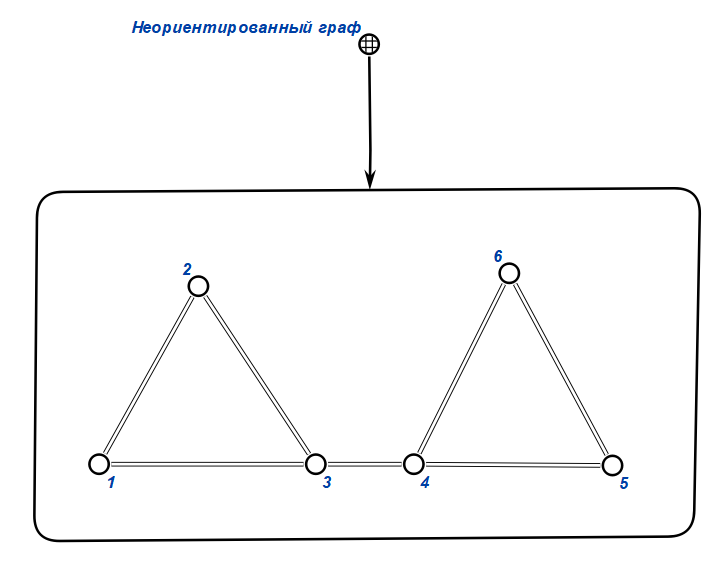
\includegraphics[width=0.58\linewidth]{Images/neorient_grapf.png}
    \caption{Неориентированный граф}
\end{figure}

Связный граф — граф, в котором существует путь между любой парой вершин. Из каждой вершины по рёбрам можно добраться до любой другой вершины. В связном графе нет изолированных вершин или групп, которые не связаны с остальными частями графа.

\begin{figure}[H]
    \centering
    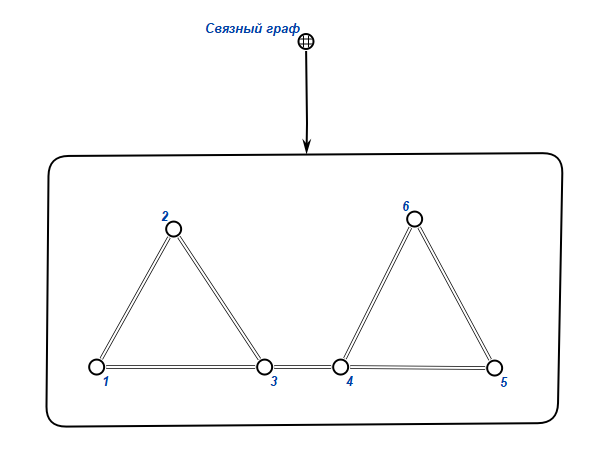
\includegraphics[width=0.58\linewidth]{Images/sv_graph.png}
    \caption{Связный граф}
\end{figure}

Несвязный граф - это граф, в котором не все вершины связаны друг с другом. Это означает, что существует по крайней мере одна пара вершин, между которыми нет пути.

\begin{figure}[H]
    \centering
    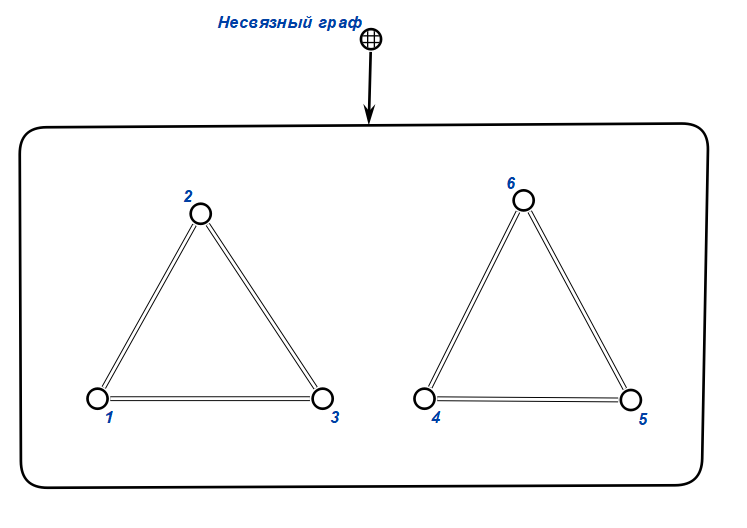
\includegraphics[width=0.58\linewidth]{Images/nesv_graph.png}
    \caption{Несвязный граф}
\end{figure}

Число реберной связности графа - это минимальное число ребер, которые нужно удалить, чтобы граф стал несвязным.

\begin{figure}[H]
    \centering
    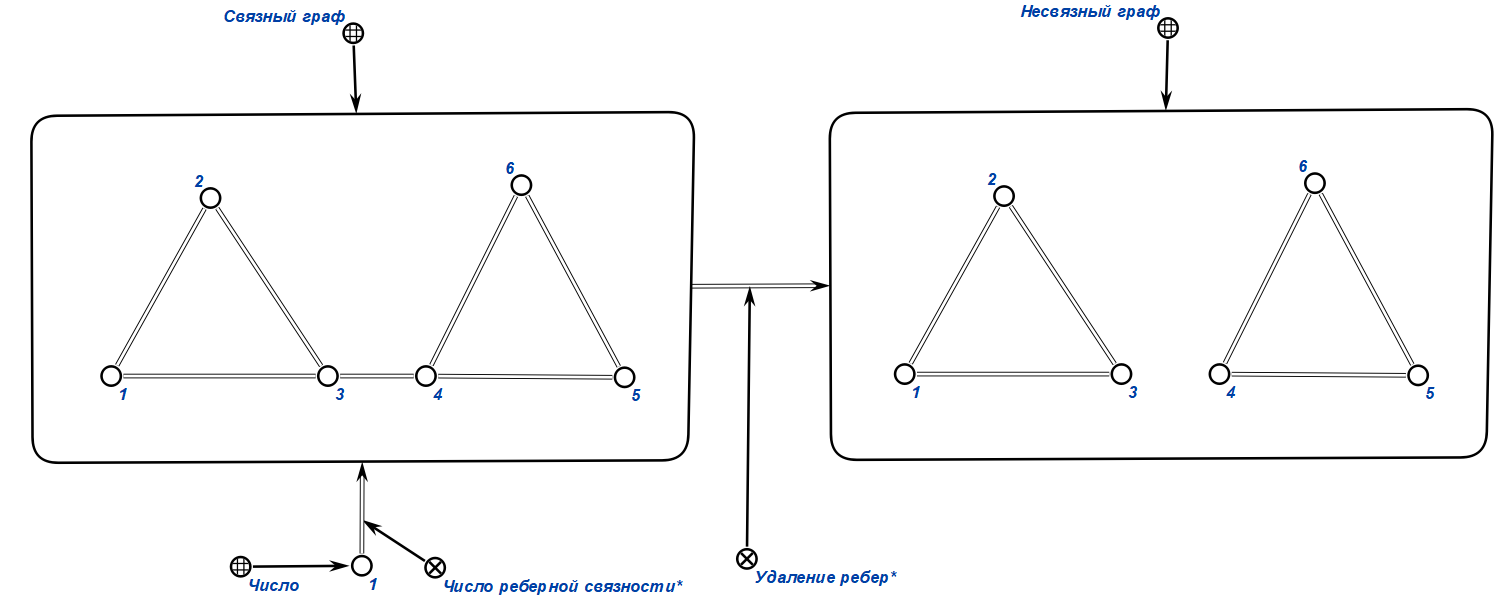
\includegraphics[width=1\linewidth]{Images/num_sv.png}
    \caption{Число реберной связности}
\end{figure}

\section{Тестовые примеры}
\subsection{Тестовый пример №1}

\begin{figure}[H]
    \centering
    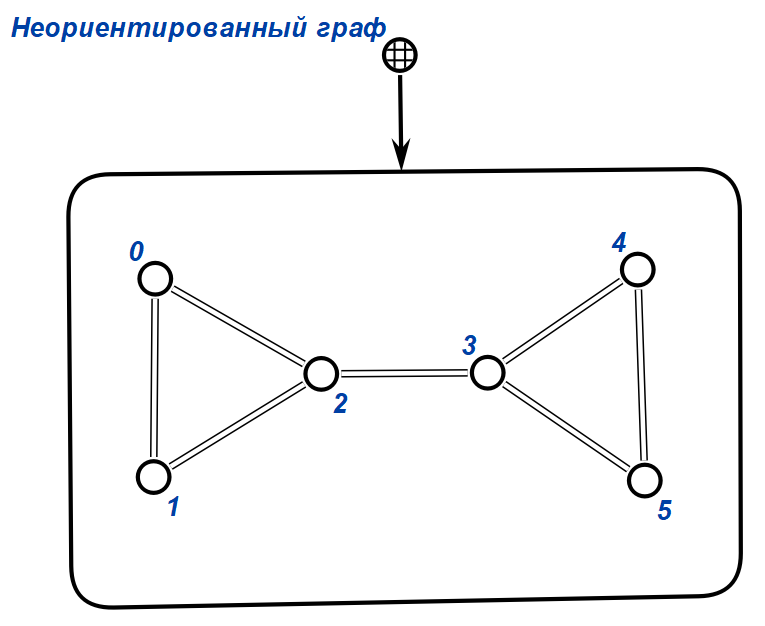
\includegraphics[width=0.58\linewidth]{Images/test_1.png}
    \caption{Неориентированный граф из тестового примера №1.}
\end{figure}

\subsection{Тестовый пример №2}

\begin{figure}[H]
    \centering
    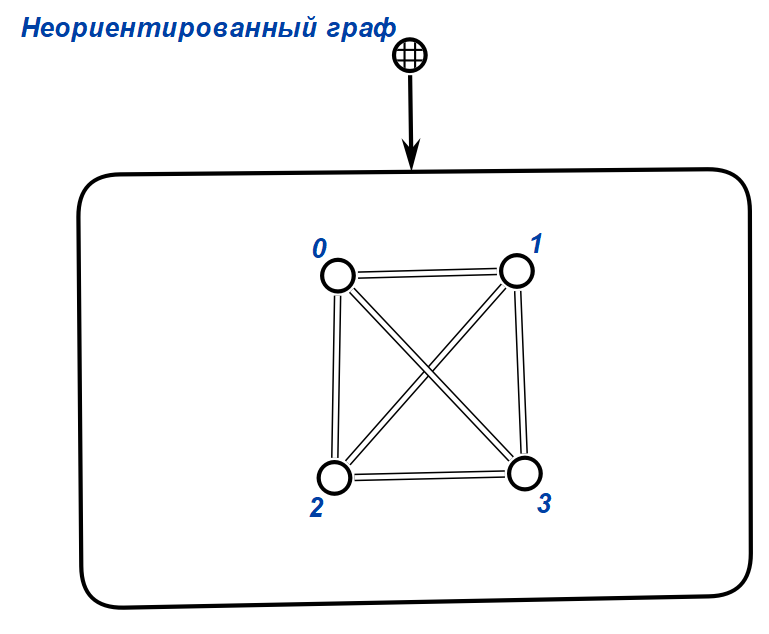
\includegraphics[width=0.58\linewidth]{Images/test_2.png}
    \caption{Неориентированный граф из тестового примера №2.}
\end{figure}

\subsection{Тестовый пример №3}

\begin{figure}[H]
    \centering
    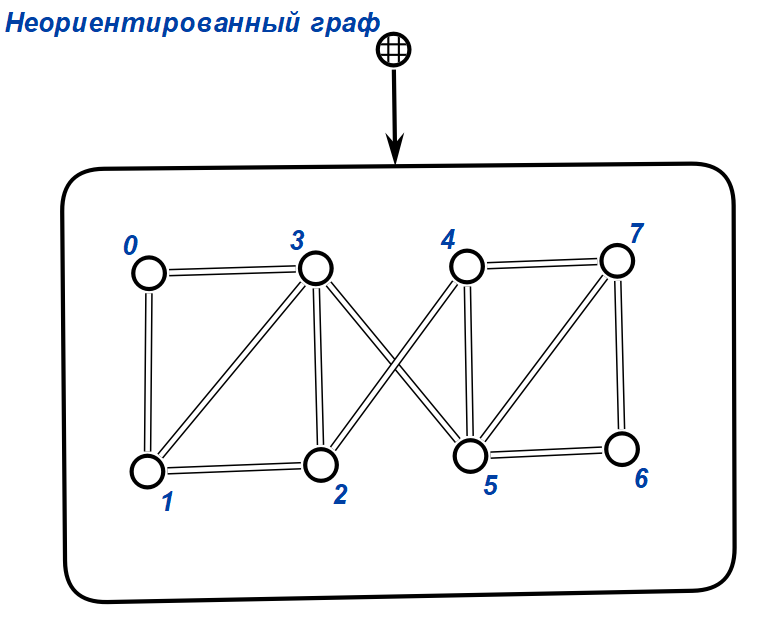
\includegraphics[width=0.58\linewidth]{Images/test_3.png}
    \caption{Неориентированный граф из тестового примера из тестового примера №3.}
\end{figure}

\subsection{Тестовый пример №4}

\begin{figure}[H]
    \centering
    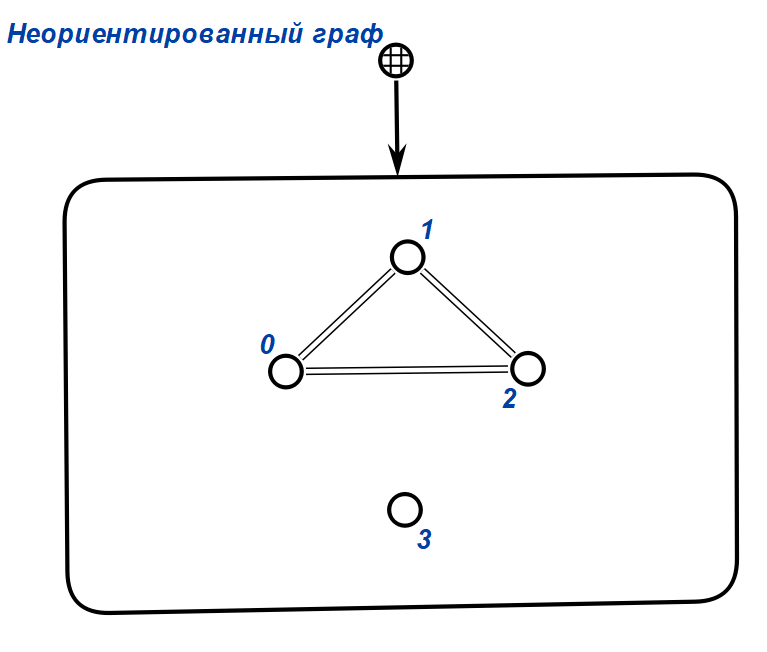
\includegraphics[width=0.58\linewidth]{Images/test_4.png}
    \caption{Неориентированный граф из тестового примера из тестового примера №4.}
\end{figure}

\subsection{Тестовый пример №5}

\begin{figure}[H]
    \centering
    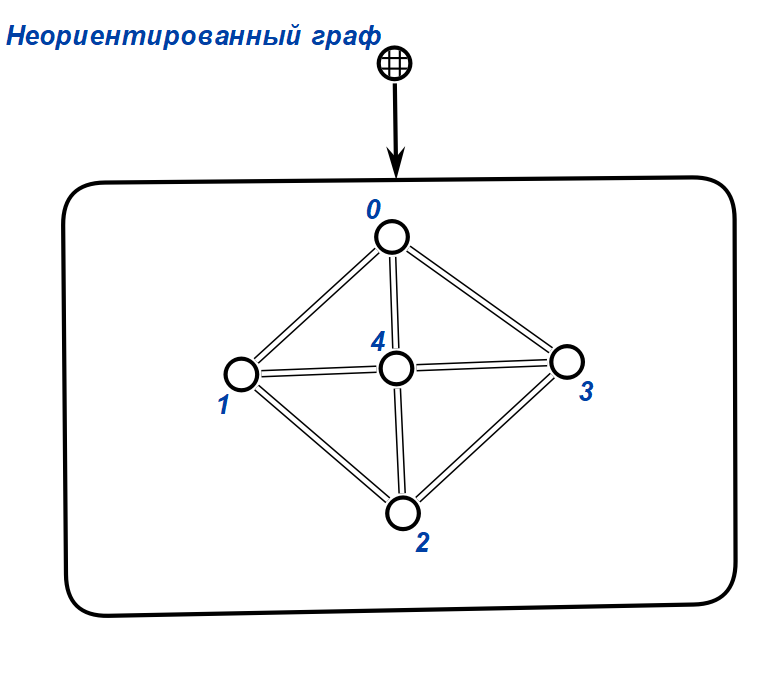
\includegraphics[width=0.58\linewidth]{Images/test_5.png}
    \caption{Неориентированный граф из тестового примера из тестового примера №5.}
\end{figure}

\section{Работа алгоритма}

\begin{enumerate}
    \item Проверить связность графа: если граф несвязный — сразу вернуть 0.

    \item Найти минимальную степень вершины: посчитать степени всех вершин (количество ребер у каждой) и взять минимальное значение. Это верхняя граница ответа.

    \item Перебрать все возможные разрезы
    для каждого непустого подмножества вершин S (кроме всего графа):
    \begin{enumerate}
        \item Вычислить дополнение: T = V / S

        \item Посчитать количество ребер между S и T

        \item Запоминать минимальное найденное значение
    \end{enumerate}

    \item Найденный минимум - число реберной связности.
\end{enumerate}

\section{Демонстрация работы алгоритма}
Работа алгоритма продемонстрируется для тестового примера №2.

\subsection{Проверка на связность}
Связный граф - это граф, из каждой вершины по рёбрам можно добраться до любой другой вершины.

\begin{figure}[H]
    \centering
    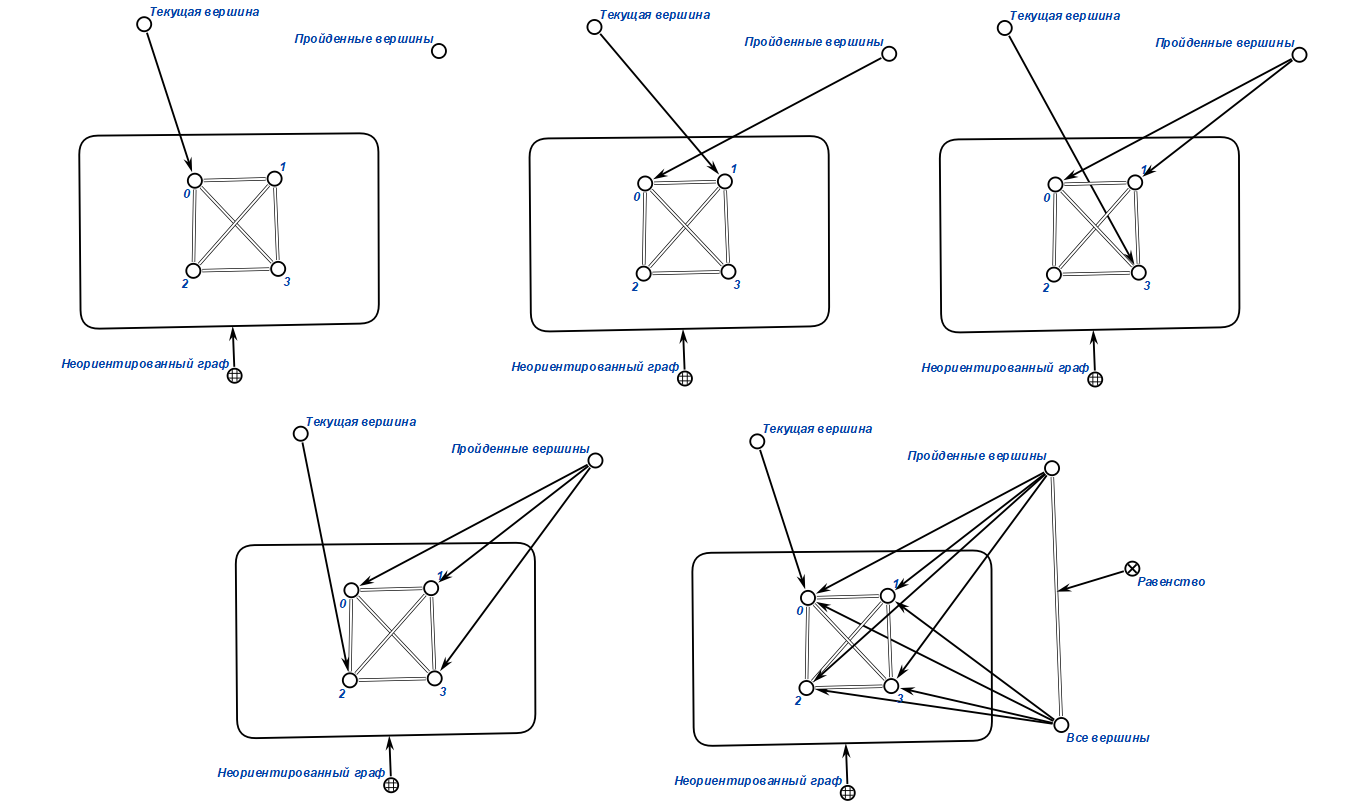
\includegraphics[width=1.0\linewidth]{Images/is_sv.png}
    \caption{Алгоритм проверки связности графа.}
\end{figure}

\subsection{Нахождение минимальной степени вершины}

Приходим к выводу, что у этого графа имеется минимально 3 ребра от каждой вершины (см. рис. 11).

\begin{figure}
    \centering
    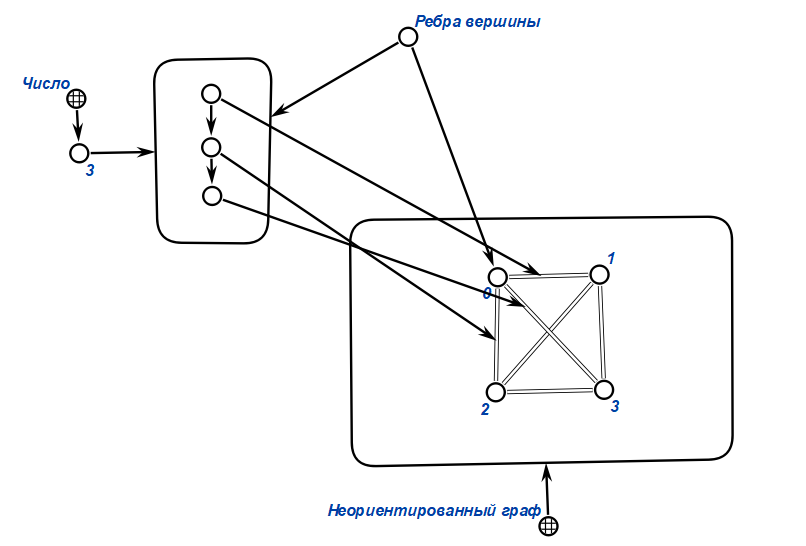
\includegraphics[width=0.5\linewidth]{Images/min_sv.png}
    \caption{Поиск числа ребер от вершины}
    \label{fig:enter-label}
\end{figure}



\subsection{Перебор возможных разрезов }

Теперь будем по очереди отсоединять вершины от графа, начиная с 1 и заканчивая 3 - минимальным числом ребер от вершины.
Сначала разрезаем граф на пары подмножеств:
\begin{enumerate}
    \item {0} - {1,2,3}
    \item {1} - {0,2,3}
    \item {2} - {0,1,3}
    \item {3} - {0,1,2}
\end{enumerate}
Теперь формируем соответствующие графы, считаем количество удаленных ребер (на рисунках показаны не все вариации).


\begin{figure}
    \centering
    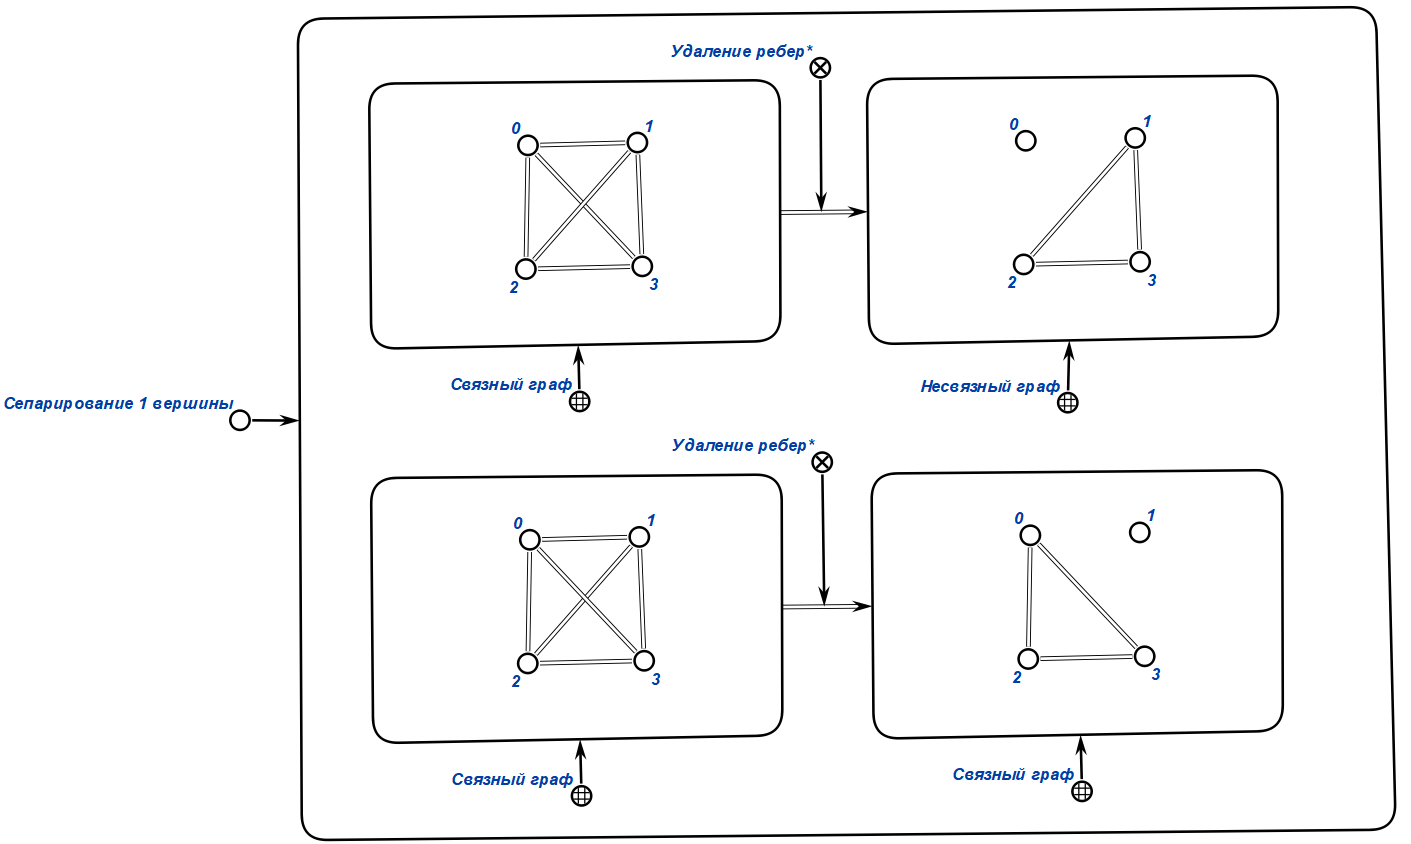
\includegraphics[width=0.8\linewidth]{Images/razb_1.png}
    \caption{Сепарация 1 вершины}
    \label{fig:enter-label}
\end{figure}


Далее разрезаем граф на следующие пары подмножеств:

\begin{figure}
    \centering
    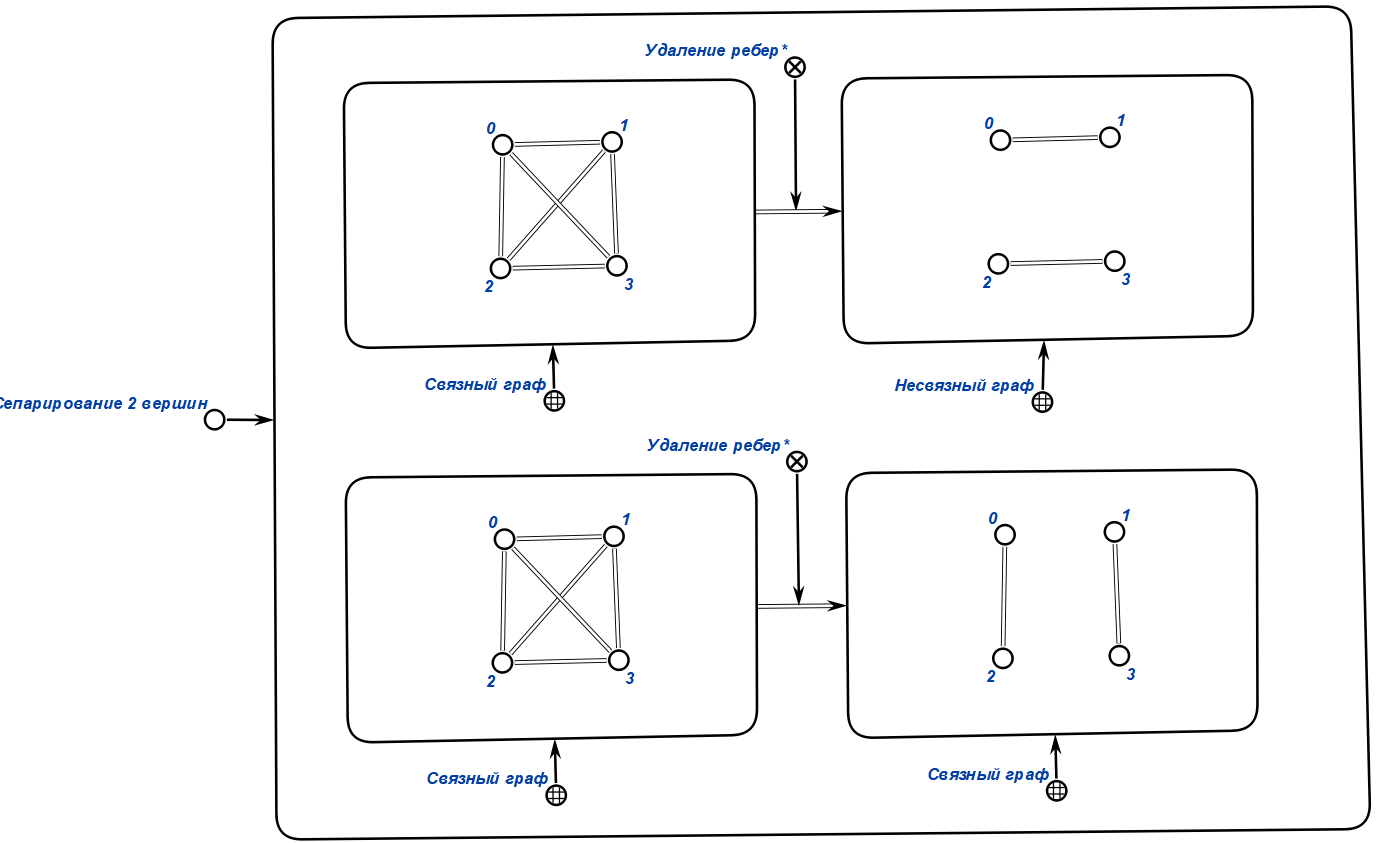
\includegraphics[width=0.8\linewidth]{Images/razb_2.png}
    \caption{Сепарация 2 вершин}
    \label{fig:enter-label}
\end{figure}

\begin{figure}
    \centering
    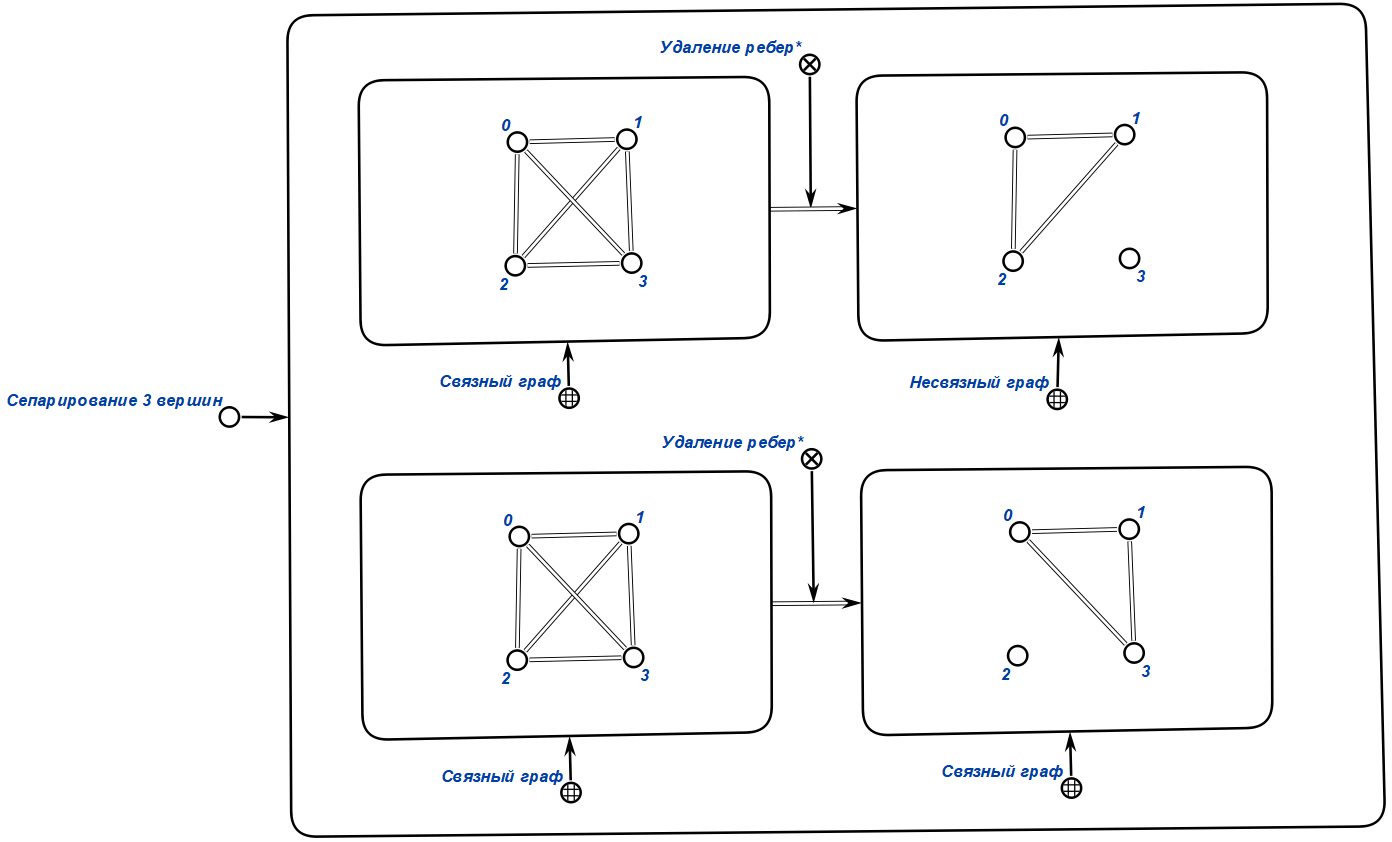
\includegraphics[width=0.8\linewidth]{Images/razb_3.png}
    \caption{Сепарация 3 вершин}
    \label{fig:enter-label}
\end{figure}


\newpage
\subsection{Результат}

Теперь осталось найти только минимальное число удаленных ребер (рис. 15).

\begin{figure}
    \centering
    
\includegraphics[width=0.5\linewidth]{Images/result.png}
    \caption{Получение результата}
    \label{fig:enter-label}
\end{figure}

\section{Заключение}
В ходе выполнения задачи пошаговой формализации алгоритма поиска числа реберной связности графа я научился формализовывать информацию с использованием семантических сетей и систематизировал знания об элементах теории графов, касающихся алгоритма поиска числа реберной связности графа.

\section{Список использованных источников}
\begin{thebibliography}{9}
\bibitem{wiki:graph}
Свободная энциклопедия <<Википедия>> [Электронный ресурс]. --- Режим доступа: \url{https://ru.wikipedia.org/wiki/Граф_(математика)}

\bibitem{brest:graphs}
Сайт <<Олимпиадное программирование в Бресте и Беларуси>> [Электронный ресурс]. --- Режим доступа: \url{https://brestprog.by/topics/graphs/}

\bibitem{habr:graphs}
Сайт <<IT-форум Хабр>> [Электронный ресурс]. --- Режим доступа:
\url{https://habr.com/ru/companies/otus/articles/568026/}
\end{thebibliography}

\end{document}